% 
%            ,,                                        
%          `7MM            _.o9                                
%            MM                                             
%  ,6"Yb.    MM  ,p6"bo   ,6"Yb.  M"""MMV  ,6"Yb.  `7Mb,od8 
% 8)   MM    MM 6M'  OO  8)   MM  '  AMV  8)   MM    MM' "' 
%  ,pm9MM    MM 8M        ,pm9MM    AMV    ,pm9MM    MM     
% 8M   MM    MM YM.    , 8M   MM   AMV  , 8M   MM    MM     
% `Moo9^Yo..JMML.YMbmd'  `Moo9^Yo.AMMmmmM `Moo9^Yo..JMML.   
% 
% 
% Free and Open-Source template for academic works
% https://github.com/dpmj/alca



\clearpage
\cleardoublepage

\chapter{Tecnologie per l'approccio distribuito ai problemi di Machine Learning}

\section{Architetture a microservizi e monolitiche}

Le architetture software rivestono un ruolo cruciale nello sviluppo e nell'implementazione di sistemi complessi. Due approcci architetturali predominanti, le architetture monolitiche e quelle a microservizi, delineano paradigmi distinti che influenzano la progettazione e la gestione dei sistemi software. La presente dissertazione si propone di analizzare dettagliatamente le differenze fondamentali tra queste due architetture, esplorando in particolare i vantaggi e gli svantaggi intrinseci all'adozione di microservizi.


Le architetture monolitiche, tradizionalmente consolidate, si caratterizzano per la centralizzazione delle funzionalità in un'unica entità. Questo modello implica che tutte le componenti del sistema siano interdipendenti, aumentando la complessità e limitando la scalabilità. Al contrario, le architetture a microservizi adottano un approccio modulare, suddividendo le funzionalità in servizi indipendenti. Questa frammentazione consente maggiore flessibilità, facilitando l'implementazione, l'aggiornamento e la manutenzione dei singoli servizi senza influire sul resto del sistema.

I vantaggi legati all'impiego di microservizi sono molteplici. In primo luogo, la modularità permette uno sviluppo più rapido e parallelo, consentendo ai team di lavoro di concentrarsi su specifiche funzionalità senza interferenze esterne. Inoltre, la scalabilità è migliorata, in quanto i singoli servizi possono essere adattati alle esigenze di carico in modo indipendente. Tuttavia, tali vantaggi non sono esenti da compromessi.

Gli svantaggi delle architetture a microservizi emergono principalmente nella complessità gestionale. La coordinazione e la gestione di numerosi servizi richiedono un'attenzione particolare, aumentando la complessità operativa complessiva. Inoltre, la distribuzione dei dati tra servizi può generare sfide in termini di coerenza e sicurezza, richiedendo un'attenta pianificazione e implementazione.

In sintesi, la scelta tra architetture monolitiche e a microservizi dipende dalle specifiche esigenze del progetto. Mentre le architetture monolitiche offrono una coesione maggiore, le architetture a microservizi forniscono flessibilità e scalabilità avanzate. Tuttavia, è essenziale ponderare attentamente i vantaggi e gli svantaggi di entrambe le opzioni al fine di adottare l'approccio più congruente con gli obiettivi e le dinamiche del sistema in questione.

L'integrazione di architetture a microservizi nell'ambito del machine learning si configura come una strategia potenzialmente vantaggiosa, in quanto si adatta in modo ottimale alle esigenze dinamiche e complesse di tali applicazioni. La natura distribuita dei microservizi si sposa bene con le peculiarità del machine learning, fornendo numerosi benefici chiave.

In primo luogo, la modularità intrinseca alle architetture a microservizi si traduce in una maggiore flessibilità e facilità di gestione delle componenti specifiche del processo di machine learning. Ogni componente del modello, come l'acquisizione dei dati, la fase di addestramento e l'inferenza, può essere implementata come un servizio separato. Ciò consente agli sviluppatori di focalizzarsi su singoli aspetti senza dover gestire l'intera complessità del sistema, agevolando così lo sviluppo, il testing e la manutenzione.

In secondo luogo, l'approccio a microservizi favorisce una maggiore scalabilità, consentendo la distribuzione indipendente di singoli servizi. Questo è particolarmente cruciale nel contesto del machine learning, dove l'addestramento di modelli può richiedere risorse computazionali significative. L'abilità di scalare in modo selettivo i servizi coinvolti nell'addestramento può portare a un utilizzo più efficiente delle risorse, migliorando le prestazioni complessive del sistema.

Un ulteriore vantaggio è la facilità di integrazione di nuove tecnologie e framework nel contesto del machine learning. La natura modulare dei microservizi consente l'aggiornamento indipendente di singoli componenti, consentendo l'adozione di nuovi algoritmi o strumenti senza dover rivedere l'intera architettura.

\begin{figure}[h]
    \centering
    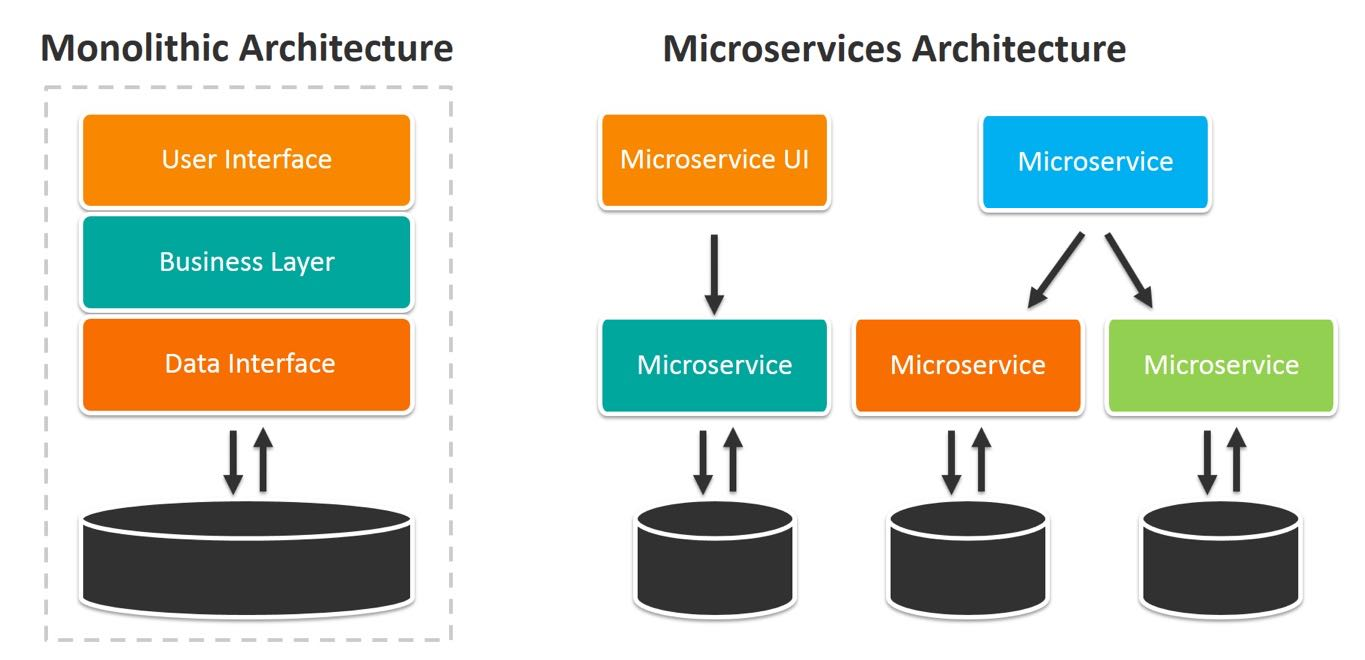
\includegraphics[width=\linewidth]{figures/ch3/micro.jpg}
    \caption[Architetture monolitiche e architetture a microservizi]{Architetture monolitiche e architetture a microservizi}
    \label{fig:cha3:microserivces}
\end{figure}

Tuttavia, è essenziale sottolineare che, sebbene le architetture a microservizi offrano numerosi vantaggi, la loro implementazione richiede una pianificazione accurata e una gestione attenta delle interazioni tra i servizi. La distribuzione di modelli di machine learning, la gestione dei dati e la sincronizzazione tra i servizi sono aspetti critici che richiedono una progettazione accurata per garantire il successo dell'implementazione a microservizi nell'ambito del machine learning.

Procediamo con un esempio pratico.

Nell'ambito di un sistema distribuito di machine learning, consideriamo un'applicazione di analisi predittiva per la manutenzione di apparecchiature industriali. Supponiamo di avere un vasto parco macchine distribuito su diverse località geografiche, ognuna dotata di sensori per monitorare le condizioni operative. L'obiettivo è prevedere guasti imminenti e pianificare la manutenzione in modo proattivo.

In questa implementazione, adottiamo un'architettura a microservizi per gestire le diverse fasi del processo di machine learning. Un servizio si occupa dell'acquisizione e dell'aggregazione dei dati provenienti dai sensori, mentre un altro servizio è dedicato all'addestramento del modello di previsione dei guasti. Il terzo servizio gestisce l'inferenza, analizzando in tempo reale i dati dei sensori e fornendo previsioni sullo stato di ciascuna macchina.

Questa suddivisione in microservizi consente uno sviluppo e una gestione agili di ciascuna componente del sistema. L'architettura distribuita facilita la scalabilità, consentendo di adattare la capacità computazionale in base alle esigenze del processo di addestramento e inferenza \cite{liu2015survey}. Inoltre, la modularità dei microservizi facilita l'integrazione di nuovi sensori o l'aggiornamento del modello di machine learning senza dover interrompere l'intero sistema \cite{yang2018microservices}.

Per garantire una maggiore affidabilità, implementiamo anche un servizio di monitoraggio della salute del sistema, che utilizza tecniche di rilevamento delle anomalie per identificare eventuali malfunzionamenti o cambiamenti nelle prestazioni \cite{ding2019using}. Questo approccio contribuisce a mantenere la stabilità del sistema distribuito nel tempo, migliorando l'affidabilità delle previsioni e riducendo il rischio di guasti imprevisti.

L'adozione di un'architettura a microservizi per un sistema distribuito di machine learning offre vantaggi significativi in termini di flessibilità, scalabilità e manutenibilità. Questo approccio si dimostra particolarmente adatto per applicazioni complesse come la manutenzione predittiva in contesti industriali, dove la gestione distribuita dei dati e dei servizi può migliorare notevolmente l'efficienza complessiva del sistema.

\section{Containerizzazione e virtualizzazione}

Il paradigma delle architetture a microservizi ha assunto una rilevanza significativa nel panorama dello sviluppo software contemporaneo, portando con sé l'ulteriore evoluzione di concetti fondamentali come containerizzazione e virtualizzazione. La distinzione tra queste due modalità di isolamento e gestione delle risorse computazionali risulta cruciale per comprendere le dinamiche che sottendono alle architetture distribuite moderne.

La virtualizzazione, inizialmente emersa come risposta alle sfide di consolidamento delle risorse hardware, presenta una struttura che coinvolge l'implementazione di macchine virtuali (VMs). Ciascuna VM opera come un'istanza indipendente di un sistema operativo ospitato su un hypervisor, fornendo un ambiente isolato e autosufficiente. Questo approccio, documentato ampiamente nella letteratura \cite{smith2005history}, ha dimostrato la sua utilità in diversi contesti, permettendo la condivisione efficiente delle risorse fisiche tra carichi di lavoro diversi.

Dall'altra parte, la containerizzazione è emersa come una modalità più leggera di isolamento delle applicazioni. I container condividono il kernel del sistema operativo sottostante, ma mantengono un ambiente isolato per l'esecuzione dell'applicazione. Questa distinzione risulta particolarmente evidente nella comparazione di Docker, uno dei runtime container più diffusi, con soluzioni di virtualizzazione come VMware. Docker è noto per la sua efficienza e agilità nell'avviare e distribuire applicazioni in contenitori, con un overhead minimo rispetto alle VMs \cite{turnbull2014docker}. Questa caratteristica di leggerezza si traduce in tempi di avvio rapidi e una gestione delle risorse più efficiente, rendendo la containerizzazione particolarmente adatta alle esigenze delle architetture a microservizi.

\begin{figure}[h]
    \centering
    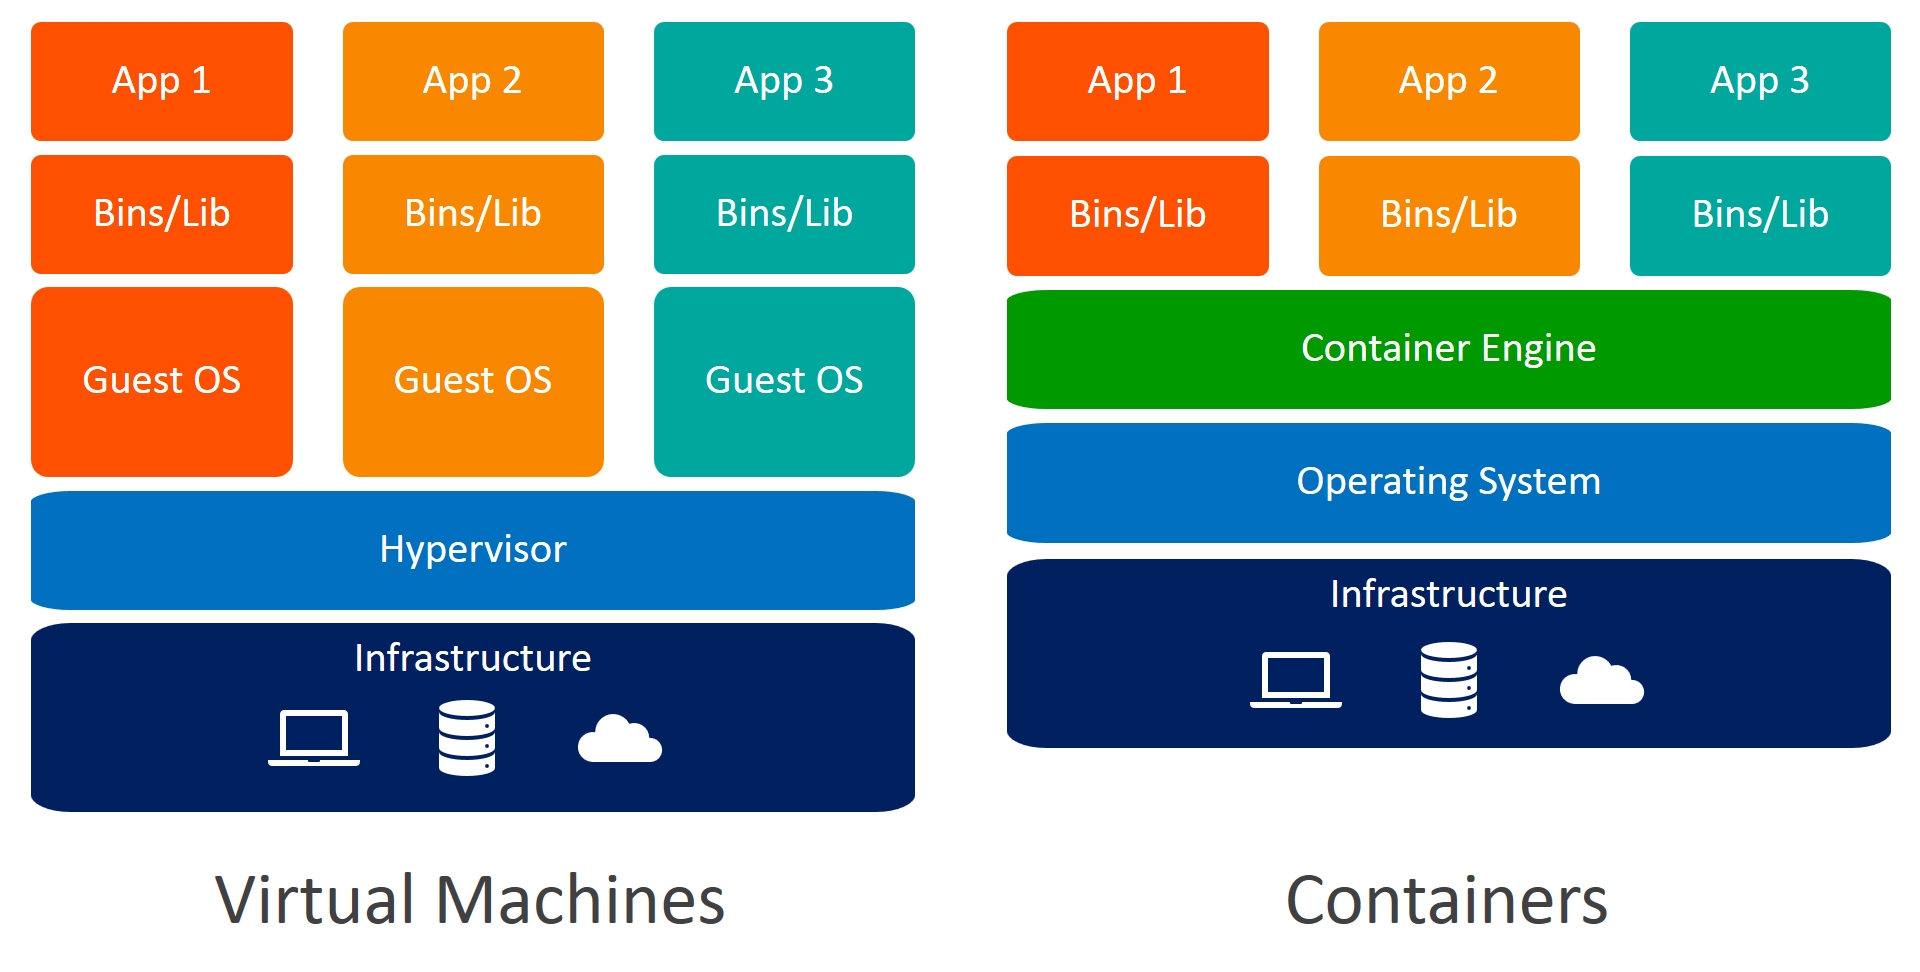
\includegraphics[width=\linewidth]{figures/ch3/containers-vs-virtualization.jpg}
    \caption[Virtualizzazione e containerizzazione]{Virtualizzazione e containerizzazione}
    \label{fig:cha3:containers}
\end{figure}

La natura modulare dei microservizi beneficia notevolmente dalla containerizzazione, poiché ciascun servizio può essere incapsulato in un contenitore autonomo. Questo facilita la distribuzione, la gestione e l'aggiornamento indipendente dei singoli componenti del sistema. La portabilità dei container, evidenziata in diverse ricerche \cite{merkel2014docker}, permette ai microservizi di essere eseguiti in modo coerente su diversi ambienti, semplificando gli ambienti di sviluppo, i test e il deployment.

L'analisi delle differenze tra containerizzazione e virtualizzazione, con un focus sull'applicabilità della containerizzazione alle architetture a microservizi, rivela la complessità e la ricchezza di queste tecnologie. La letteratura scientifica offre una base solida per comprendere i principi di entrambe le approcci, mentre il ruolo cruciale di Docker e di altri runtime container nell'ambito della containerizzazione conferma la rilevanza pratica di tali concetti nelle attuali dinamiche di sviluppo e deployment delle applicazioni.

L'approfondimento delle dinamiche che collegano la containerizzazione alle architetture a microservizi rivela ulteriori ragioni per cui questa sinergia è diventata preponderante nel panorama dello sviluppo software moderno. Le architetture a microservizi sono intrinsecamente caratterizzate da una modularità che facilita la scalabilità e la manutenzione indipendente dei singoli servizi. La containerizzazione, con la sua capacità di isolare e confezionare le applicazioni in unità leggere e autosufficienti, si allinea perfettamente con questo paradigma.

La gestione efficiente delle dipendenze e delle librerie, attraverso l'inclusione di tutto ciò che è necessario all'interno del container, elimina molte delle sfide tipiche legate alla distribuzione di applicazioni complesse. La standardizzazione fornita dai container agevola l'implementazione di best practices come la continuous integration e continuous deployment (CI/CD), accelerando il ciclo di sviluppo e riducendo il rischio di errori durante le fasi di distribuzione \cite{fowler2013continuous}.

Un altro aspetto significativo è la flessibilità nell'utilizzo di tecnologie eterogenee all'interno di un'unica applicazione a microservizi. Ciascun servizio può essere sviluppato e distribuito indipendentemente, utilizzando il linguaggio di programmazione o il framework più adatto alle specifiche esigenze. La containerizzazione, in questo contesto, agisce come un'interfaccia standardizzata, consentendo l'esecuzione di servizi eterogenei su una stessa infrastruttura \cite{burns2016borg}.

Infine, la gestione dinamica dei container, come esemplificato negli orchestration tools come \glsname{kubernetes}, si presta magnificamente alla natura scalabile e dinamica delle architetture a microservizi. La scalabilità orizzontale dei singoli servizi è agevolata dalla facilità con cui i container possono essere replicati e distribuiti su nodi multipli \cite{burns2016borg}. Ciò si traduce in una maggiore resilienza del sistema, in grado di adattarsi automaticamente alle variazioni del carico di lavoro.

L'intreccio tra containerizzazione e architetture a microservizi rappresenta un punto focale nel panorama dello sviluppo software contemporaneo. La leggerezza, la portabilità e la gestione dinamica dei container si combinano in modo sinergico con i principi di modularità e indipendenza delle architetture a microservizi, delineando una prospettiva intrinsecamente adatta per soddisfare le esigenze delle applicazioni moderne e distribuite. La vasta letteratura su questo argomento testimonia l'entusiasmo e l'interesse crescenti che questa sinergia ha suscitato nella comunità scientifica e industriale.

\subsection{Docker}

L'adozione di Docker, nell'ambito della containerizzazione, riveste una rilevanza tecnologica cruciale, offrendo un livello di astrazione che va oltre la virtualizzazione tradizionale. Un'analisi attenta dei meccanismi sottostanti a Docker svela un approccio sofisticato alla creazione, gestione e distribuzione di contenitori leggeri e autosufficienti.

Iniziamo esaminando il processo di creazione di un container Docker. Docker utilizza un concetto chiave chiamato Dockerfile, che rappresenta un manifesto dichiarativo per la configurazione del container. All'interno di questo file, gli sviluppatori definiscono le istruzioni passo dopo passo per creare l'ambiente di esecuzione desiderato, specificando le dipendenze, i comandi di avvio e altro ancora. Questa metodologia dichiarativa consente la riproducibilità e la consistenza tra ambienti di sviluppo, test e produzione \cite{turnbull2014docker}.

Un aspetto fondamentale di Docker è la gestione efficiente delle risorse del sistema. Docker Engine utilizza la tecnologia di namespaces e cgroups del kernel Linux per isolare e limitare le risorse dei container, garantendo una coesistenza armoniosa su un sistema host condiviso. Questa implementazione si traduce in un overhead minimo rispetto alle tradizionali VMs, rendendo Docker particolarmente adatto a scenari di sviluppo e deployment agili \cite{merkel2014docker}.

\begin{figure}[h]
    \centering
    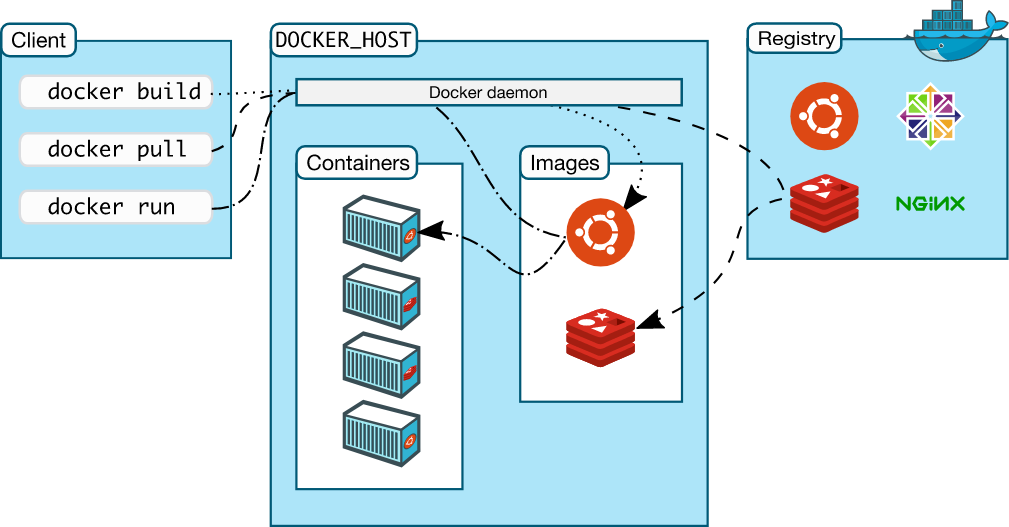
\includegraphics[width=\linewidth]{figures/ch3/docker-example.png}
    \caption[Esempio di un tipico impiego di Docker]{Esempio di un tipico impiego di Docker}
    \label{fig:cha3:docker}
\end{figure}

Nel contesto delle architetture a microservizi, Docker assume un ruolo centrale nella creazione di unità modulari. Ciascun microservizio può essere incapsulato in un container autonomo, fornendo un'interfaccia standardizzata per l'esecuzione indipendente. L'utilizzo di Docker Compose, uno strumento che permette di definire e gestire multi-container Docker applications, semplifica ulteriormente l'orchestrazione di più servizi in ambienti complessi \cite{boettiger2015introduction}.

L'aspetto della portabilità rappresenta un altro tratto distintivo di Docker. La struttura dei container Docker, che incorpora l'applicazione insieme alle sue dipendenze e librerie, consente il facile spostamento tra ambienti eterogenei. La standardizzazione dei container semplifica la distribuzione su diversi ambienti, riducendo le discrepanze tra lo sviluppo, il testing e la produzione \cite{turnbull2014docker}.

Infine, l'evoluzione del concetto di orchestrazione dei container ha visto l'emergere di strumenti come Kubernetes, che si integrano sinergicamente con Docker. Kubernetes facilita la gestione dinamica dei container, consentendo la distribuzione, l'aggiornamento e la scalabilità orizzontale dei container Docker in un ambiente di produzione \cite{burns2016borg}.

In conclusione, l'analisi tecnica di Docker rivela una comprensione approfondita delle sue funzionalità e del suo impatto nelle moderne pratiche di sviluppo e deployment. L'integrazione di Docker nelle architetture a microservizi offre una soluzione tecnologica avanzata, evidenziata dalla sua capacità di fornire isolamento efficiente, gestione ottimizzata delle risorse e portabilità delle applicazioni. La vasta adozione di Docker nella comunità dello sviluppo software testimonia della sua efficacia nel soddisfare le esigenze di un ambiente tecnologico in continua evoluzione.
